Para organizar as atividades de desenvolvimento deste projeto, optamos por utilizar
a metodologia ágil \textbf{Scrum}. Com ela, foi possível dividir as entregas em tarefas
específicas, acompanhar o progresso do time e garantir o cumprimento dos prazos
definidos.
\medskip


\noindent{As tarefas foram organizadas em três colunas principais:}
\begin{itemize}[itemsep=0.6em, topsep=0.3em, parsep=0pt]
    \item \textbf{Pendente}:  Tarefas ainda não iniciadas;
    \item \textbf{Em Progresso}: Tarefas que estão sendo desenvolvidas no momento;
    \item \textbf{Concluído}: Tarefas já finalizadas pela equipe.
\end{itemize}
\medskip

\begin{figure}[H]
\centering
\caption{Quadro Scrum com tarefas do projeto}%
\label{fig:quadro-scrum}
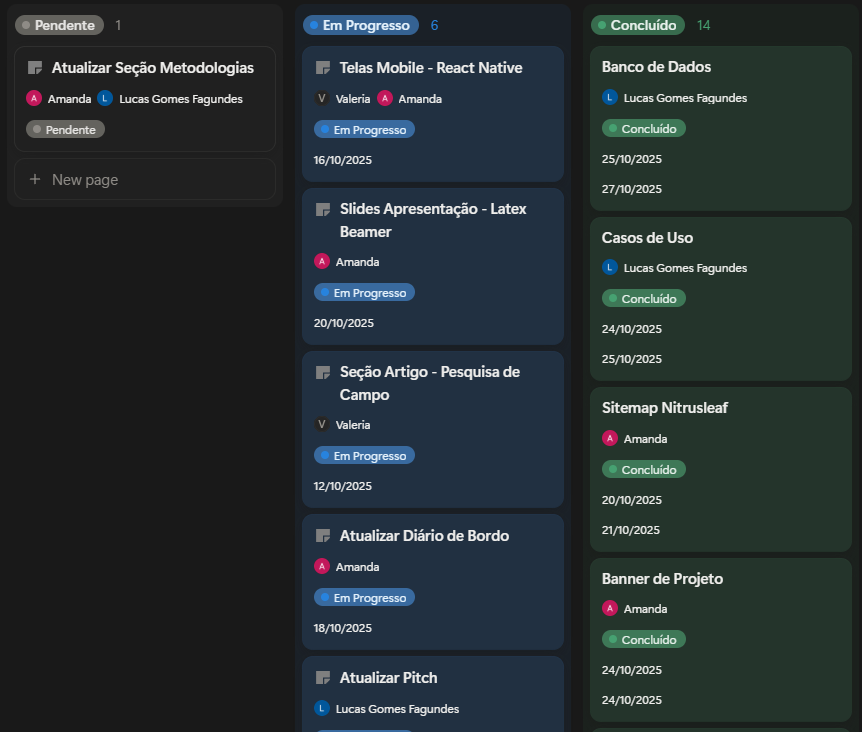
\includegraphics[width=0.8\textwidth]{Images/Scrum.png}
\SourceOrNote{Equipe 21 - Vitalliz (2025)}
\end{figure}
\medskip

Cada atividade foi priorizada conforme sua urgência e atribuída aos membros
responsáveis. Essa abordagem nos permitiu manter o foco, colaborar de forma
eficiente e adaptar o projeto conforme as necessidades surgiam ao longo do tempo.
